\section{Фильтр Калмана}
Рассмотрим систему: 
\begin{equation}
    \begin{cases}
        \dot{x} = Ax + f \\ 
        y = Cx + \xi
    \end{cases}, \quad x_0 = \begin{bmatrix}1 & 1 & 1 & 1\end{bmatrix}^T
\end{equation}
где $f(t)$ и $\xi(t)$ -- некоторый гауссовский шум с известной дисперсией и мат. ожиданием. 
\begin{equation}
    \begin{array}{ccc}
        A = \begin{bmatrix}
            -40 & 16 & 9 & 7 \\ 
            -64 & 25 & 14 & 12 \\ 
            -26 & 11 & 7 & 3 \\ 
            -48 & 18 & 14 & 8
        \end{bmatrix}, & 
        C = \begin{bmatrix}
            -3 \\ 2 \\ -2 \\ 1
        \end{bmatrix}^T
    \end{array}
\end{equation}
\begin{equation}
    Var(f) = 0.4,  \quad E(f) = 0, \quad Var(\xi) = 0.2,  \quad  E(\xi) = 0
\end{equation}
\subsection{Наблюдаемость собственных чисел}
Для определения наблюдаемости собственных чисел рассмотрим вещественную Жорданову форму системы:
\begin{equation}
    \begin{array}{ll}
        \dot{\hat{x}} = P^{-1}AP\hat{x}\\
        \hat{y} = C\hat{x}
    \end{array}
\end{equation}
Где $P$ -- матрица собственных векторов матрицы $A$, а $\hat{x} = P^{-1}x$.
\begin{equation}
    \begin{array}{ccc}
        \begin{bmatrix}
            -0.00  & -2.00  & 0.00  & 0.00 \\ 
            2.00  & 0.00  & 0.00  & 0.00 \\ 
            0.00  & 0.00  & -0.00  & -3.00 \\ 
            0.00  & 0.00  & 3.00  & 0.00 \\ 
        \end{bmatrix}, &
        P = \begin{bmatrix}
            1.14  & -0.05  & 1.13  & 0.14 \\ 
            1.74  & -0.22  & 1.84  & 0.14 \\ 
            0.87  & -0.11  & 0.71  & 0.00 \\ 
            1.41  & 0.00  & 1.41  & 0.00 \\ 
        \end{bmatrix}, & 
        C_j =\begin{bmatrix}
            -0.27 \\ -0.05  \\ 0.28  \\ -0.14 \\ 
        \end{bmatrix}^T
    \end{array}
\end{equation}
Таким образом, система является полностью наблюдаемой. 

\subsection{Синтез фильтра Калмана}
Рассмотрим наблюдатель:
\begin{equation}
    \begin{array}{ll}
        \dot{\hat{x}} = A\hat{x} + L(\hat{y} - y) \\
    \end{array}
\end{equation}
Зададимся четырьмя матрицами весов $Q$ и $R$ для синтеза фильтра Калмана:
\begin{equation}
    Q_1 = 2\cdot I_{4\times4}, \quad
    R_1 = 2
\end{equation}
\begin{equation}
    Q_2 = 2\cdot I_{4\times4}, \quad
    R_2 = 20
\end{equation}
\begin{equation}
    Q_3 = 20\cdot I_{4\times4}, \quad
    R_3 = 2
\end{equation}
\begin{equation}
    Q_4 = 20\cdot I_{4\times4}, \quad
    R_4 = 20
\end{equation}

На основе этих матриц будем синтезировать фильтр Калмана, минимизирующий критерий доверия $J$:
\begin{equation}
    J = \int_0^\infty \left( fQ^{-1}f + \xi R^{-1}\xi \right) dt
\end{equation}
Для получения фильтра Калмана необходимо решить уравнение Риккати при $v = 1$: 
\begin{equation}
    \begin{cases}
        AP + PA^T + Q - vPC^TR^{-1}CP = 0 \\
        L = -PC^TR^{-1}
    \end{cases}
\end{equation}

Для каждой пары матриц весов $Q_i$ и $R_i$ получаем фильтр Калмана, минимизирующий критерий доверия $J$: 
\begin{equation}
    \begin{array}{ccccc}
        L_1 = 
        \begin{bmatrix}
        5.63 \\ 
        6.71 \\ 
        3.63 \\ 
        5.38 \\ 
        \end{bmatrix} & 
        L_2 = 
        \begin{bmatrix}
        0.72 \\ 
        0.46 \\ 
        0.56 \\ 
        0.47 \\ 
        \end{bmatrix} &
        L_3 = 
        \begin{bmatrix}
        29.08 \\ 
        39.46 \\ 
        18.63 \\ 
        30.44 \\ 
        \end{bmatrix} & 
        L_4 = 
        \begin{bmatrix}
        5.63 \\ 
        6.71 \\ 
        3.63 \\ 
        5.38 \\ 
        \end{bmatrix} 
    \end{array}
\end{equation}
\subsection{Моделирование}
Проведем моделирование системы с фильтром Калмана $L_i$ и начальными условиями $x(0) = \begin{bmatrix} 1 & 1 & 1 & 1 \end{bmatrix}^T$ для 
системы и $\hat{x}(0) = \begin{bmatrix} 0 & 0 & 0 & 0 \end{bmatrix}^T$ для фильтра. Схема моделирования представлена на рисунке \ref{fig:kalman_scheme}.
\begin{figure}[ht!]
    \centering
    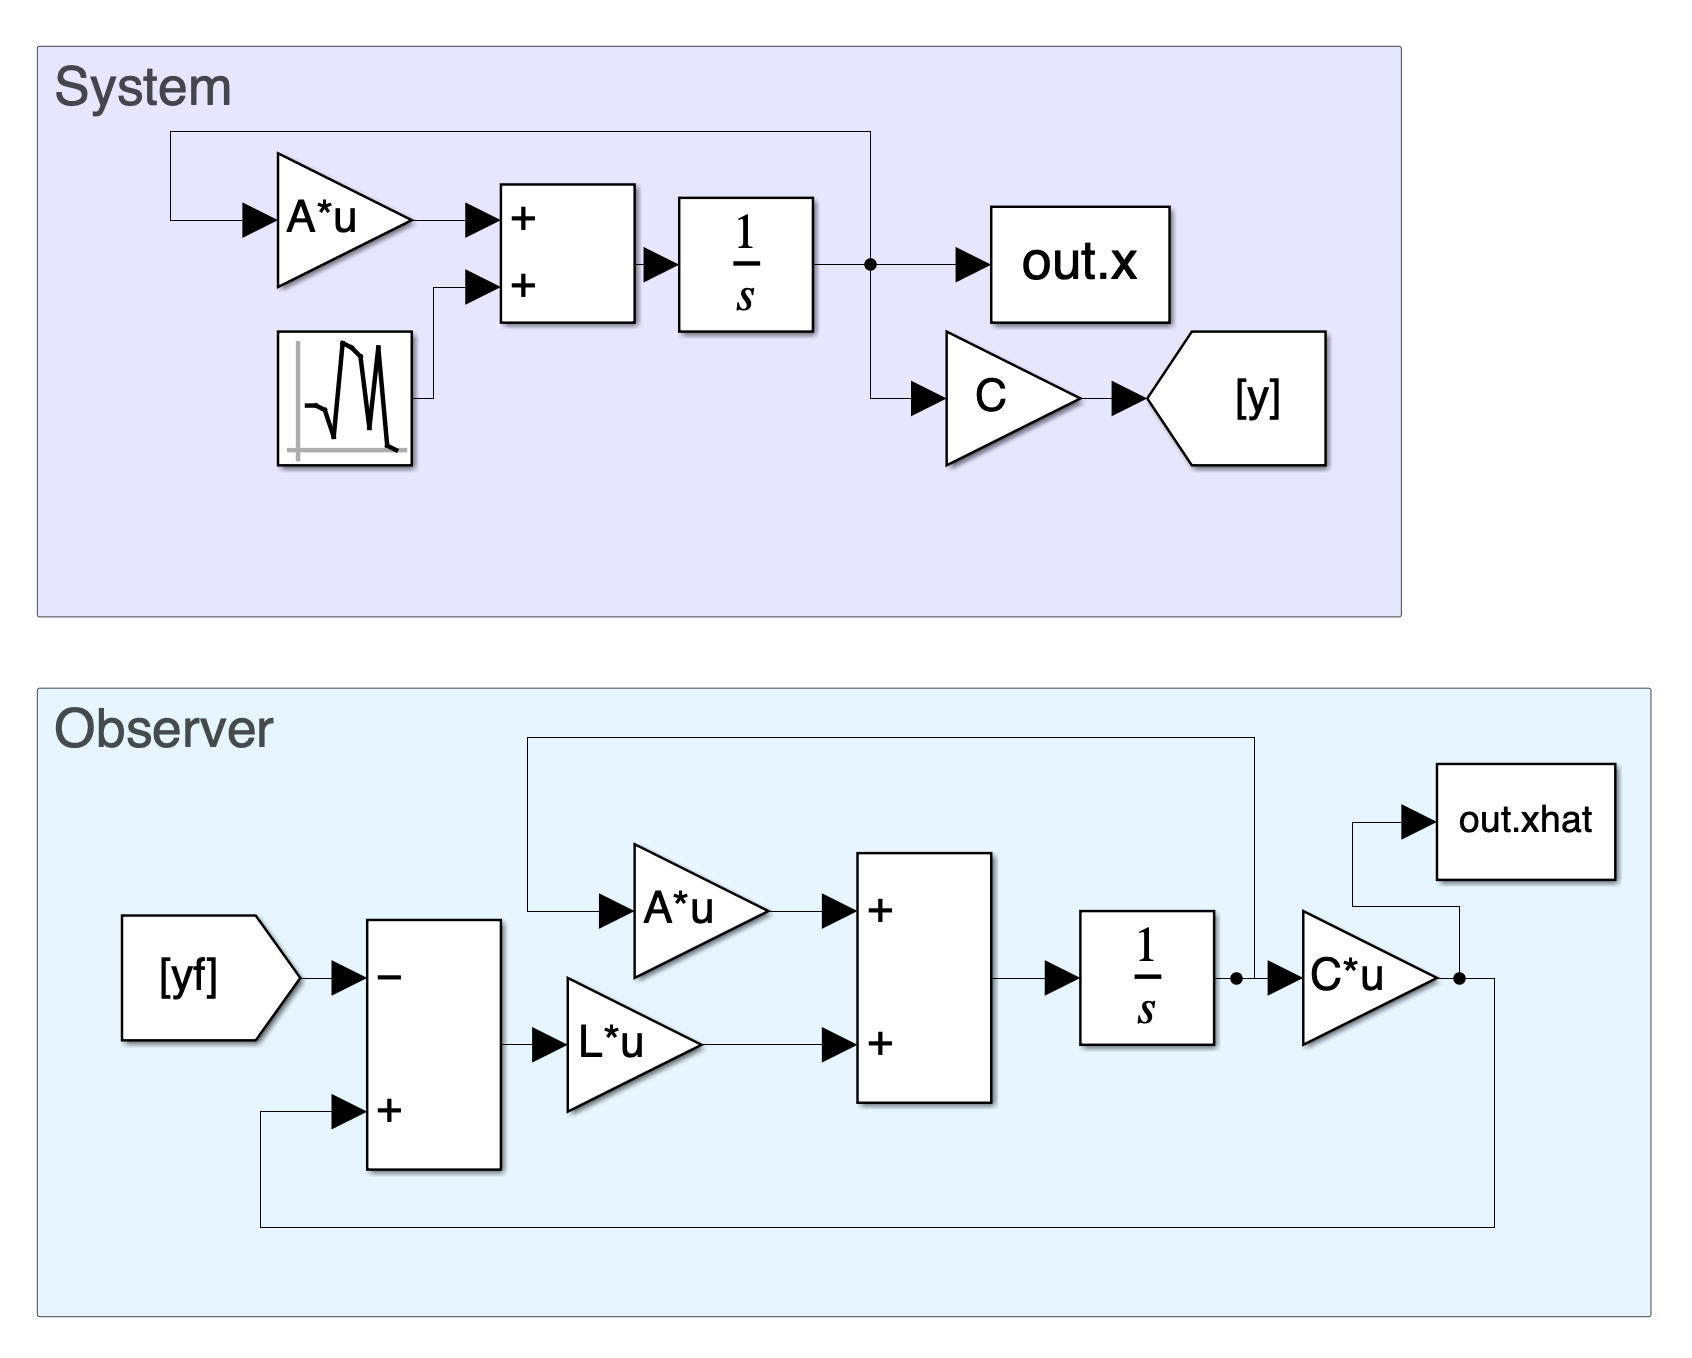
\includegraphics[width=0.8\textwidth]{media/kalman_scheme.png}
    \caption{Схема моделирования фильтра Калмана}
    \label{fig:kalman_scheme}
\end{figure}
Результаты моделирования представлены на рисунках \ref{fig:kalman1_y} (выход системы с шумом и без),
\ref{fig:kalman1_x} -- \ref{fig:kalman4_x} (векторы состояния системы и векторы оценки состояния фильтром Калмана), 
\ref{fig:kalman1_err} -- \ref{fig:kalman4_err} (ошибки оценки состояния фильтром Калмана). 
\begin{figure}[ht!]
    \centering
    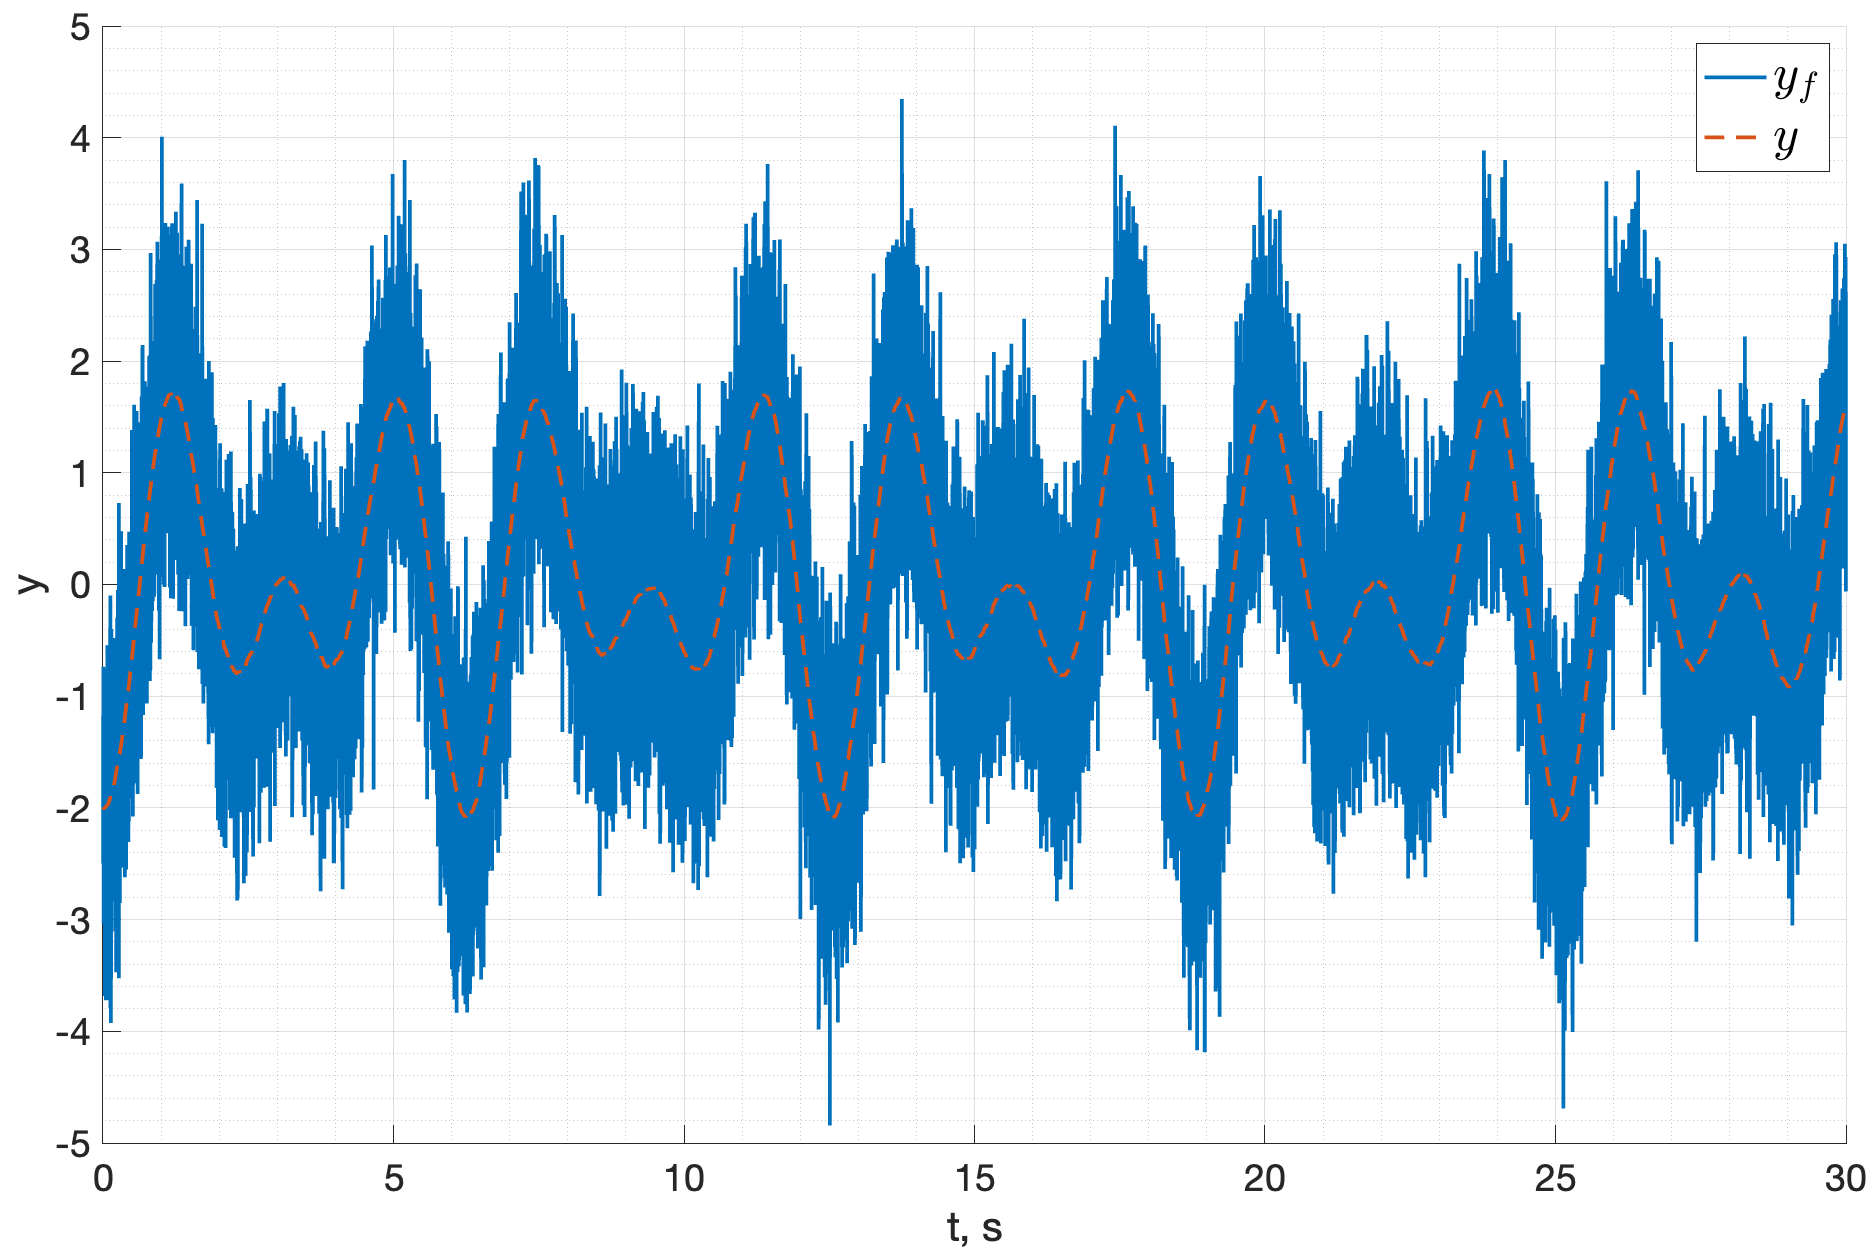
\includegraphics[width=\textwidth]{media/plots/kalman_task2/y_cmp_1.png}
    \caption{Сравнение выходов системы с шумом и без} 
    \label{fig:kalman1_y}
\end{figure}

\begin{figure}[ht!]
    \centering
    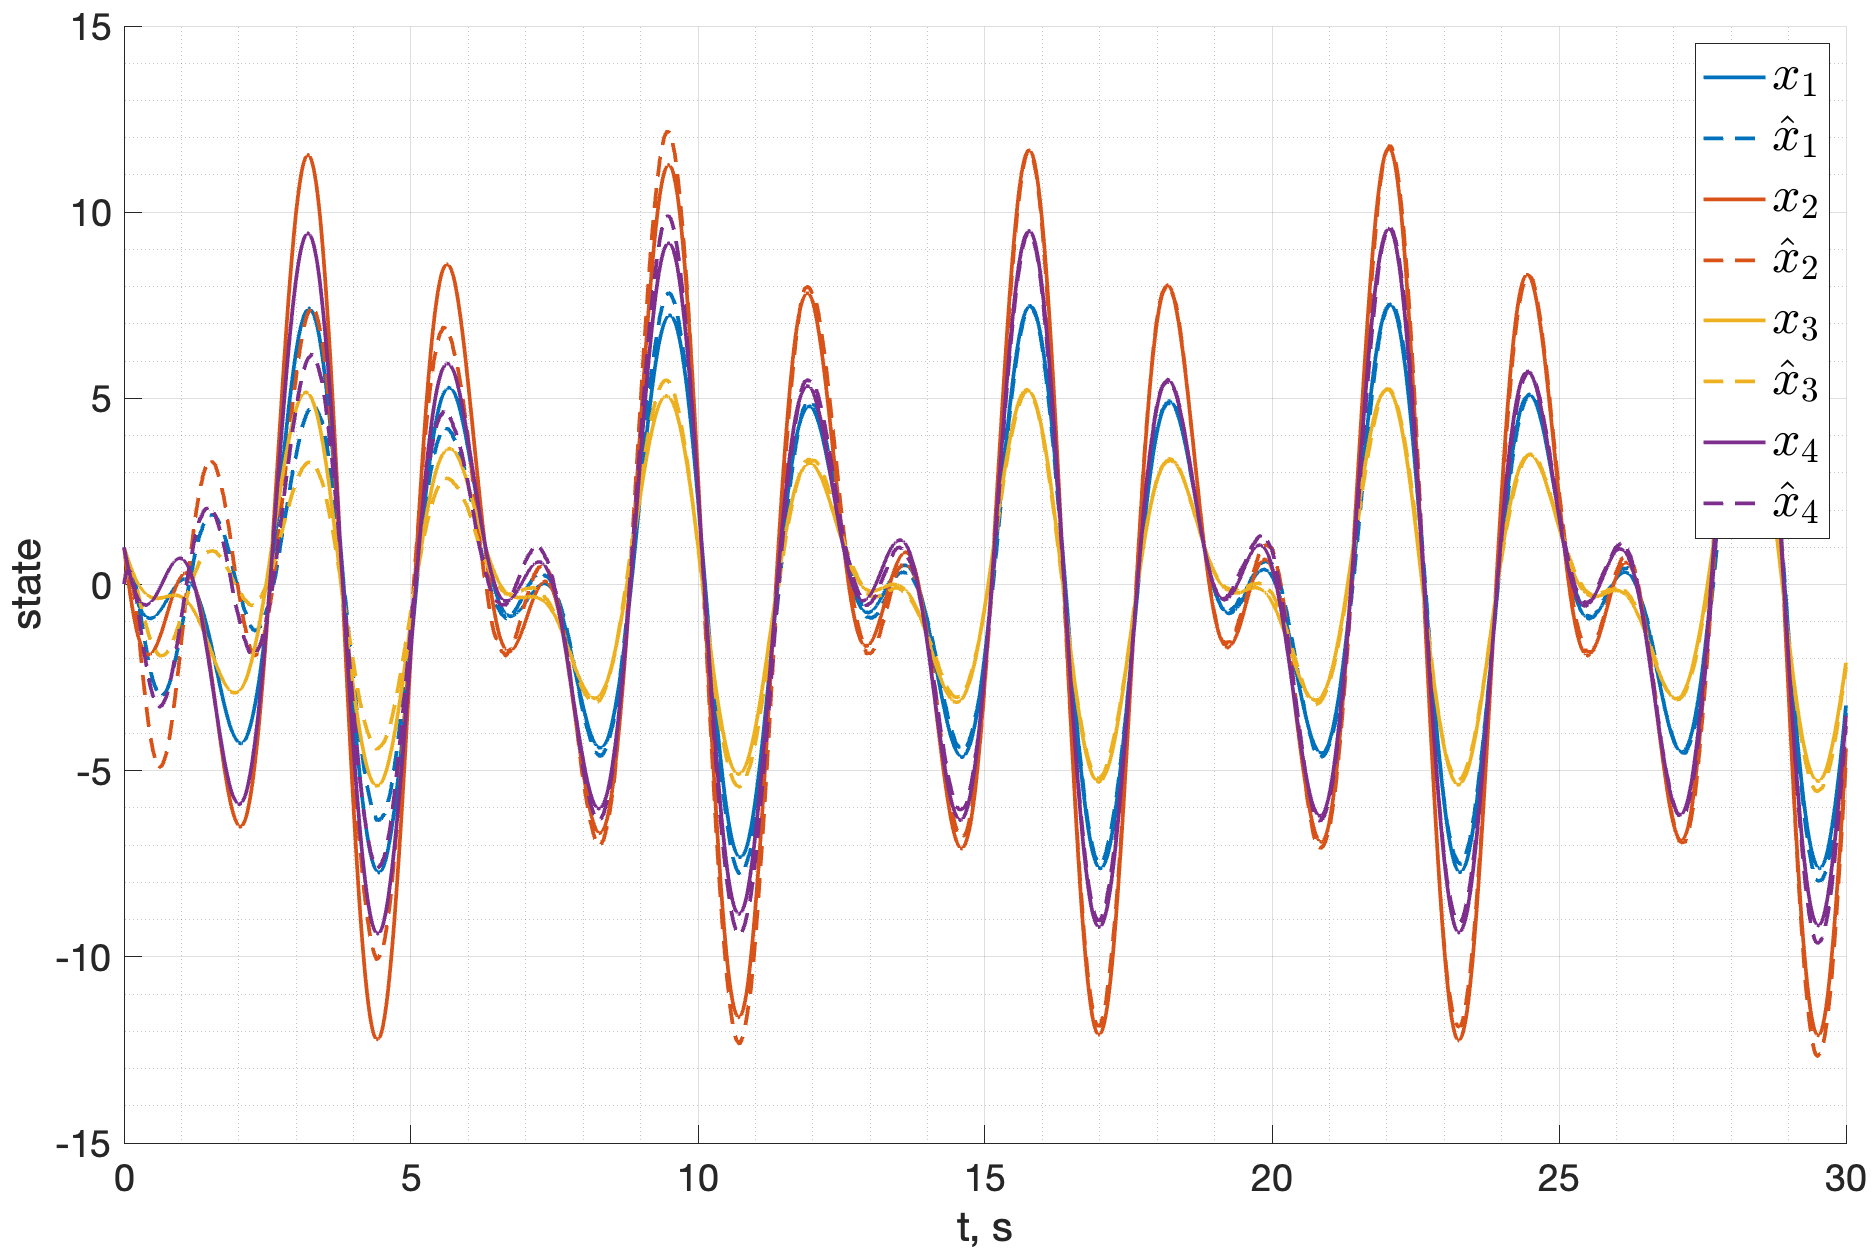
\includegraphics[width=\textwidth]{media/plots/kalman_task2/state_cmp_1.png}
    \caption{Сравнение векторов состояния системы и оценки состояния фильтром Калмана $L_1$}
    \label{fig:kalman1_x}
\end{figure}
\begin{figure}[ht!]
    \centering
    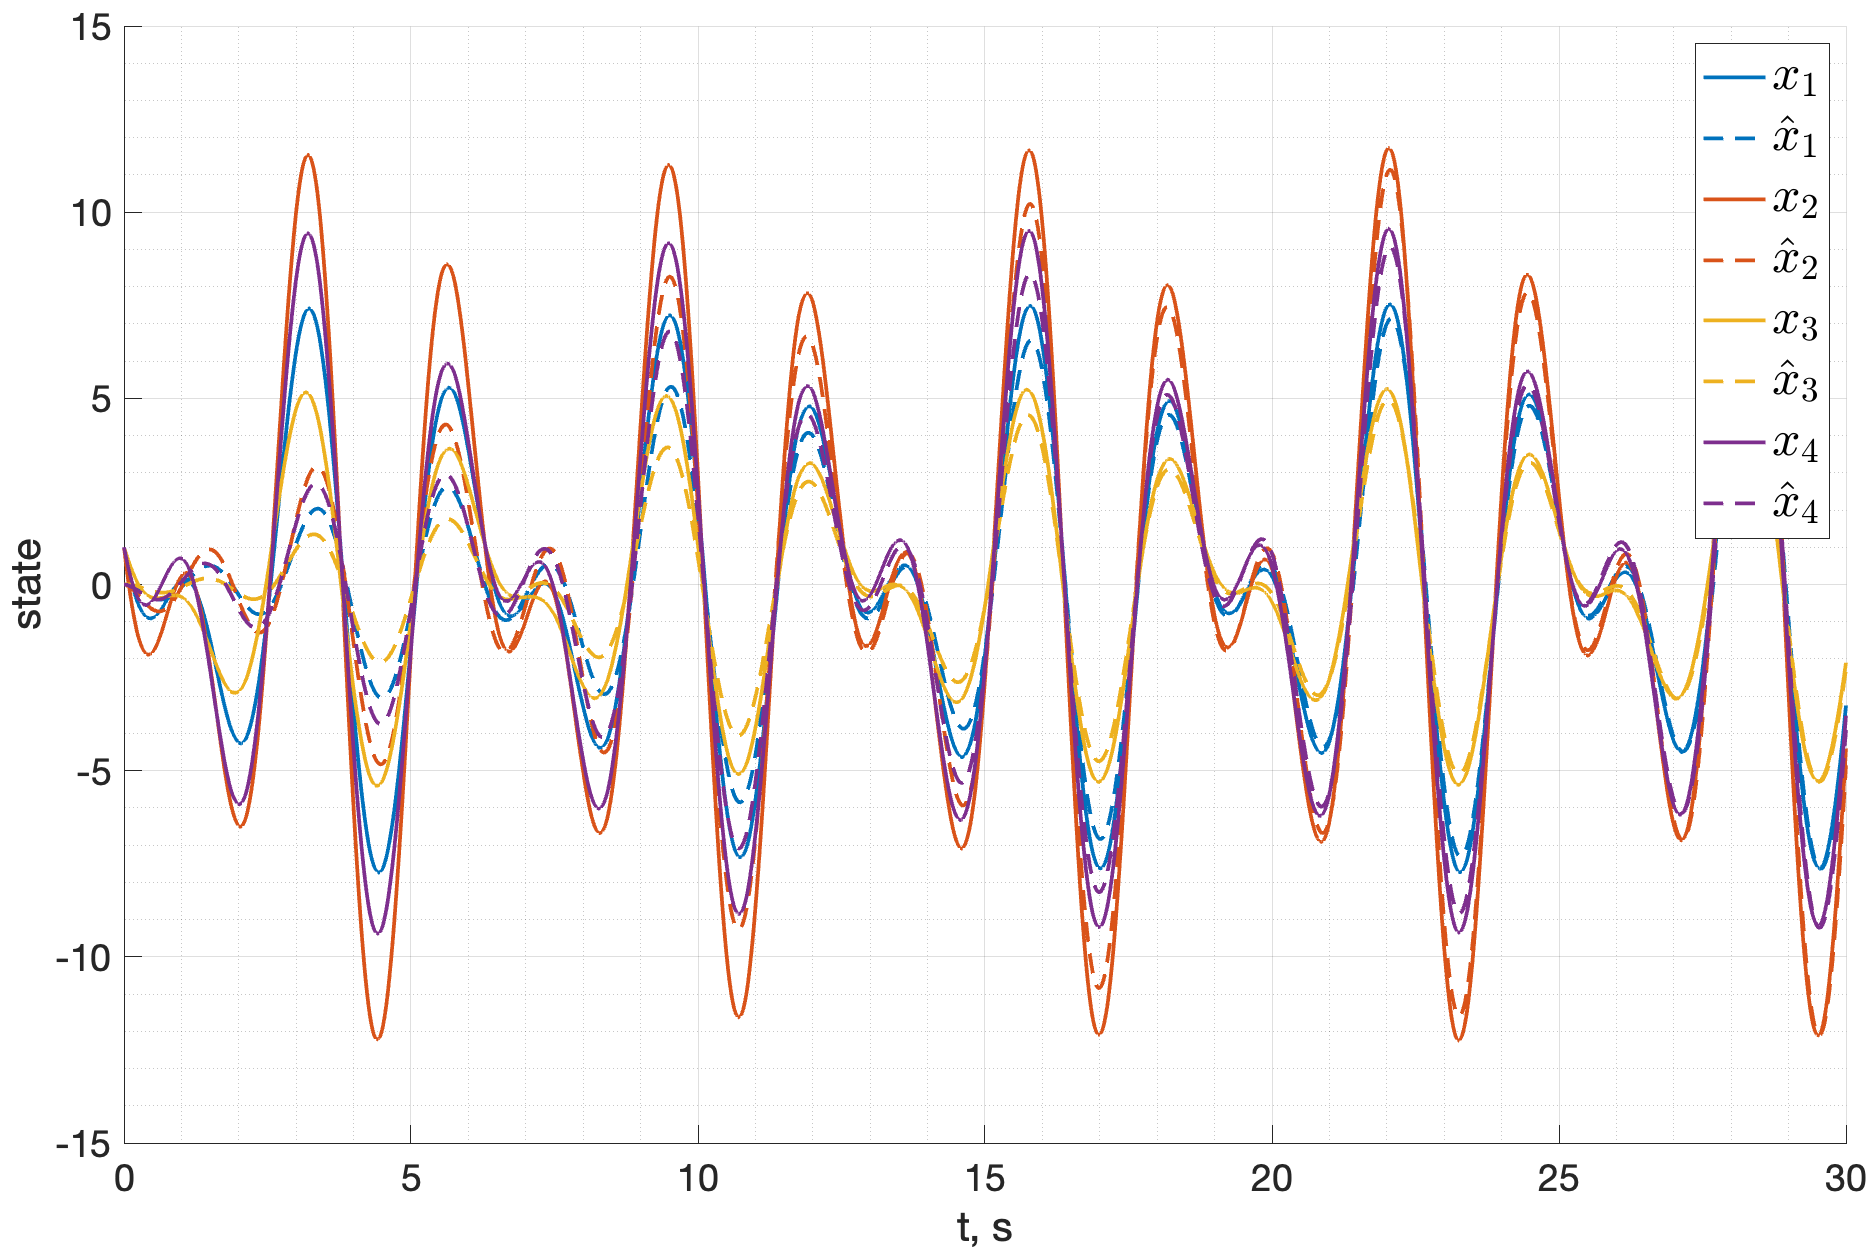
\includegraphics[width=\textwidth]{media/plots/kalman_task2/state_cmp_2.png}
    \caption{Сравнение векторов состояния системы и оценки состояния фильтром Калмана $L_2$}
    \label{fig:kalman2_x}
\end{figure}
\begin{figure}[ht!]
    \centering
    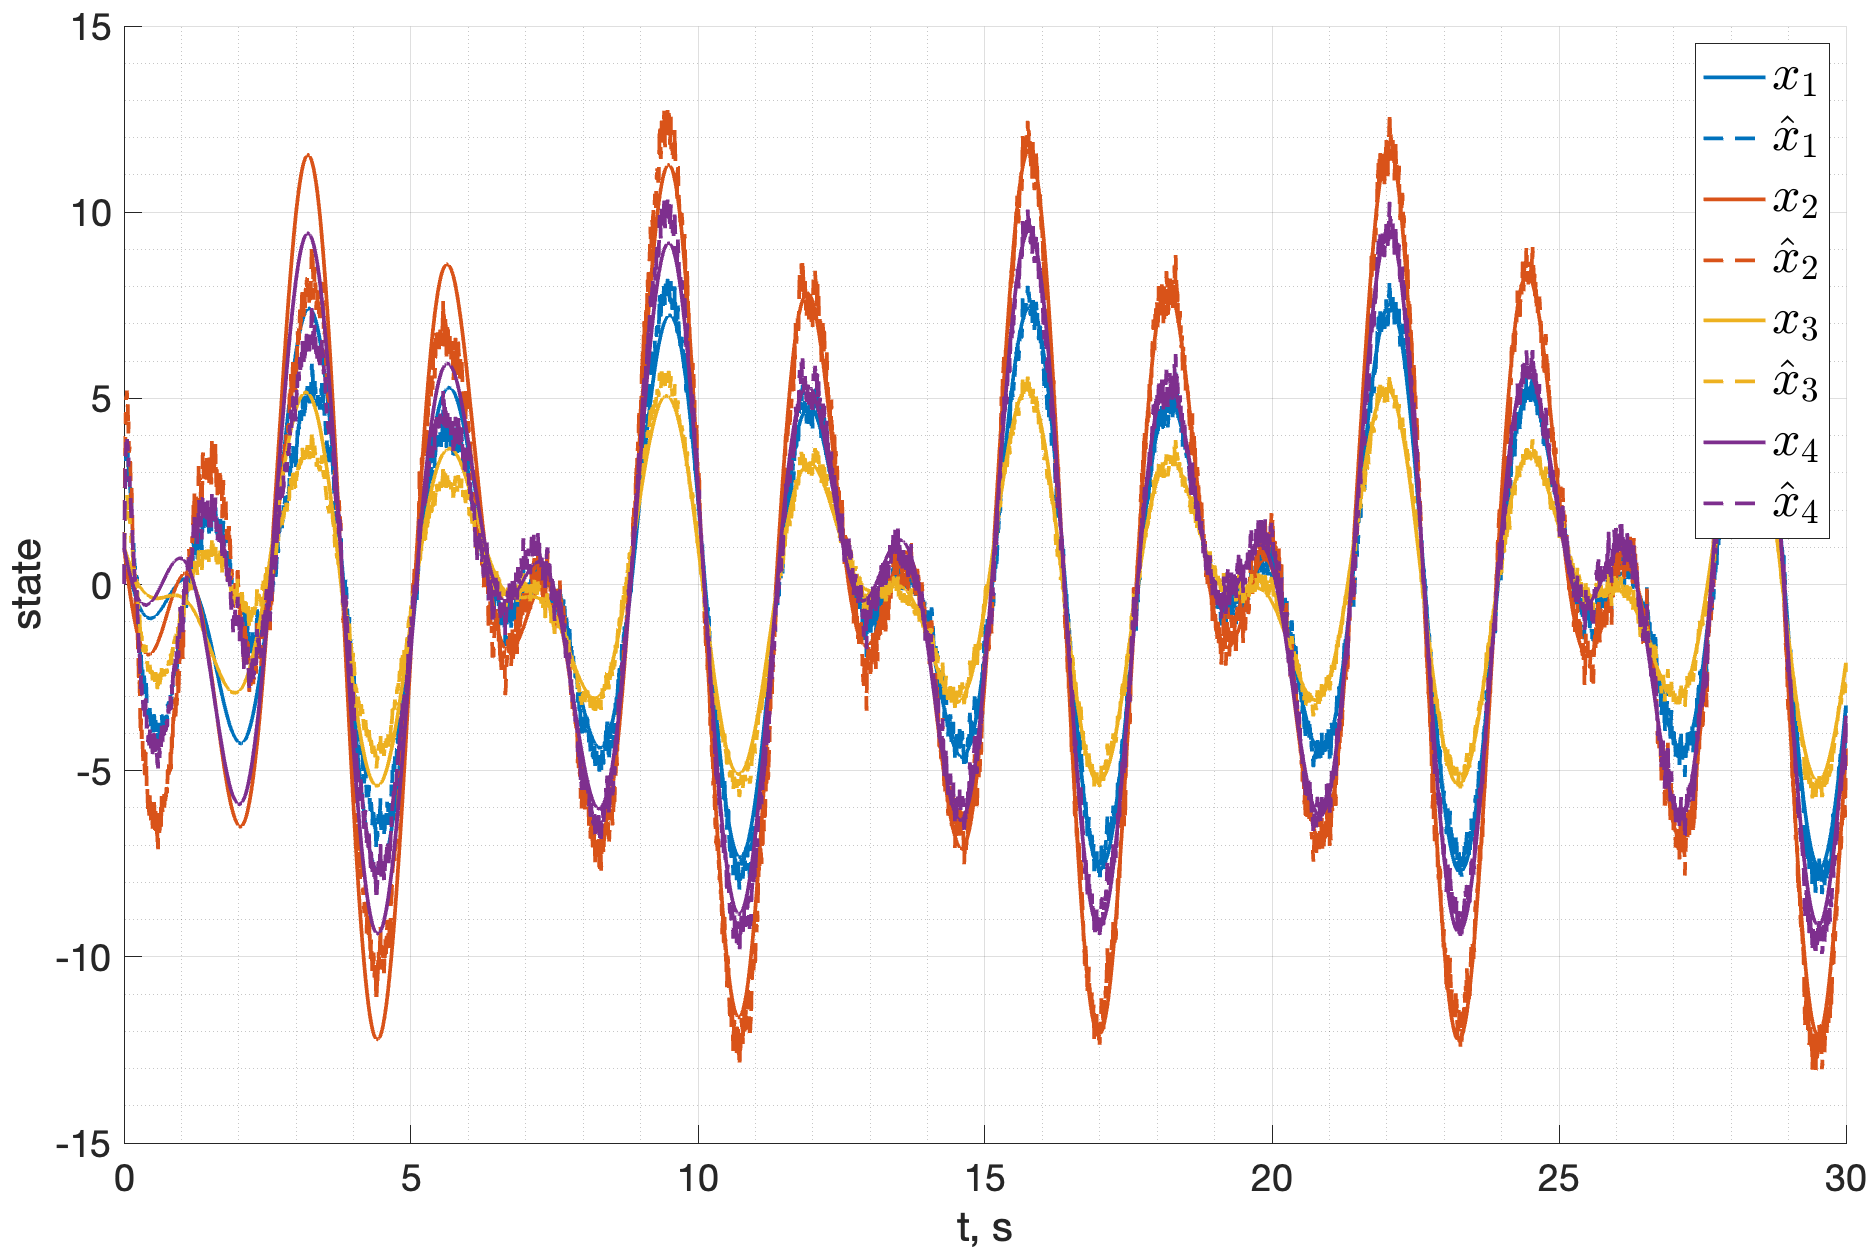
\includegraphics[width=\textwidth]{media/plots/kalman_task2/state_cmp_3.png}
    \caption{Сравнение векторов состояния системы и оценки состояния фильтром Калмана $L_3$}
    \label{fig:kalman3_x}
\end{figure}
\begin{figure}[ht!]
    \centering
    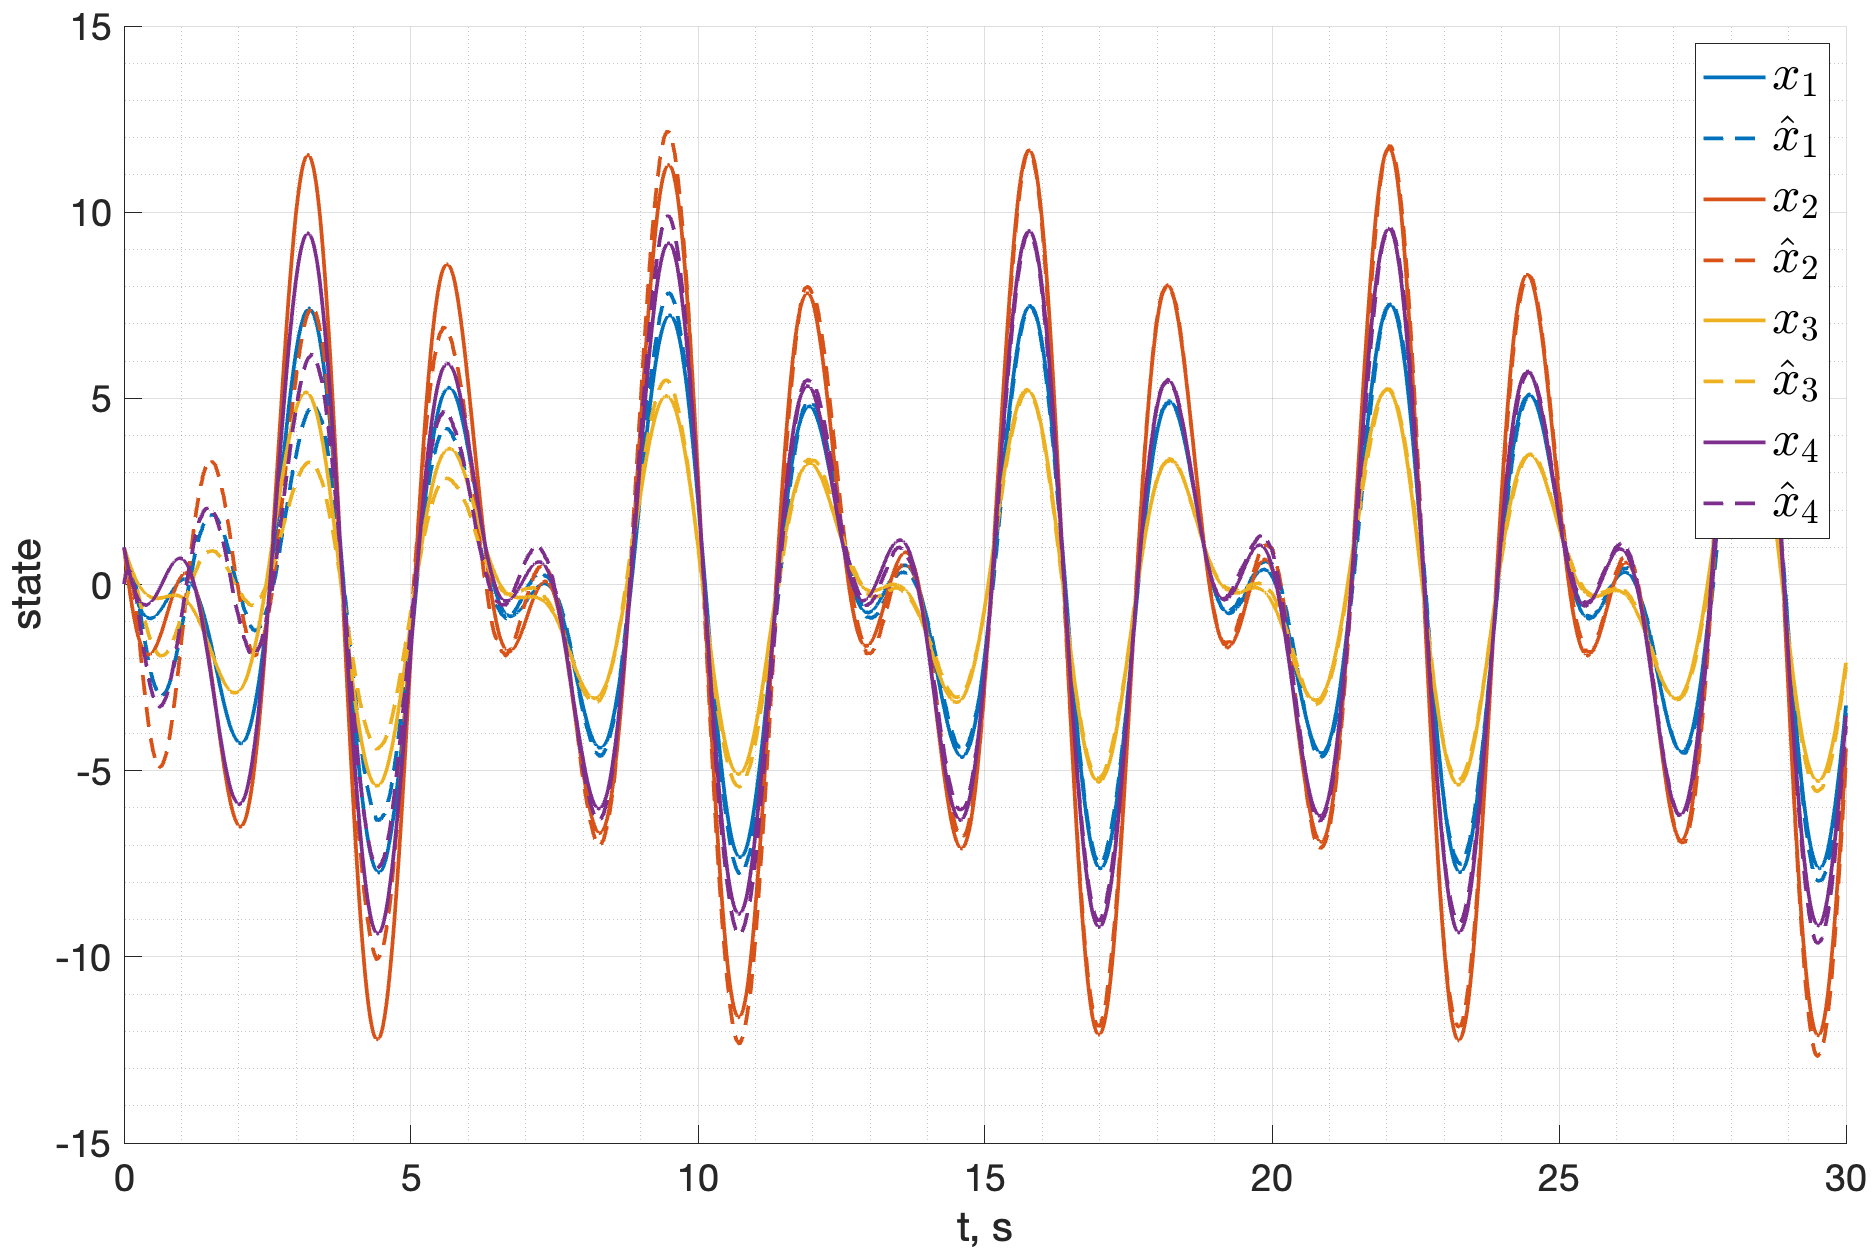
\includegraphics[width=\textwidth]{media/plots/kalman_task2/state_cmp_4.png}
    \caption{Сравнение векторов состояния системы и оценки состояния фильтром Калмана $L_4$}
    \label{fig:kalman4_x}
\end{figure}

\begin{figure}[ht!]
    \centering
    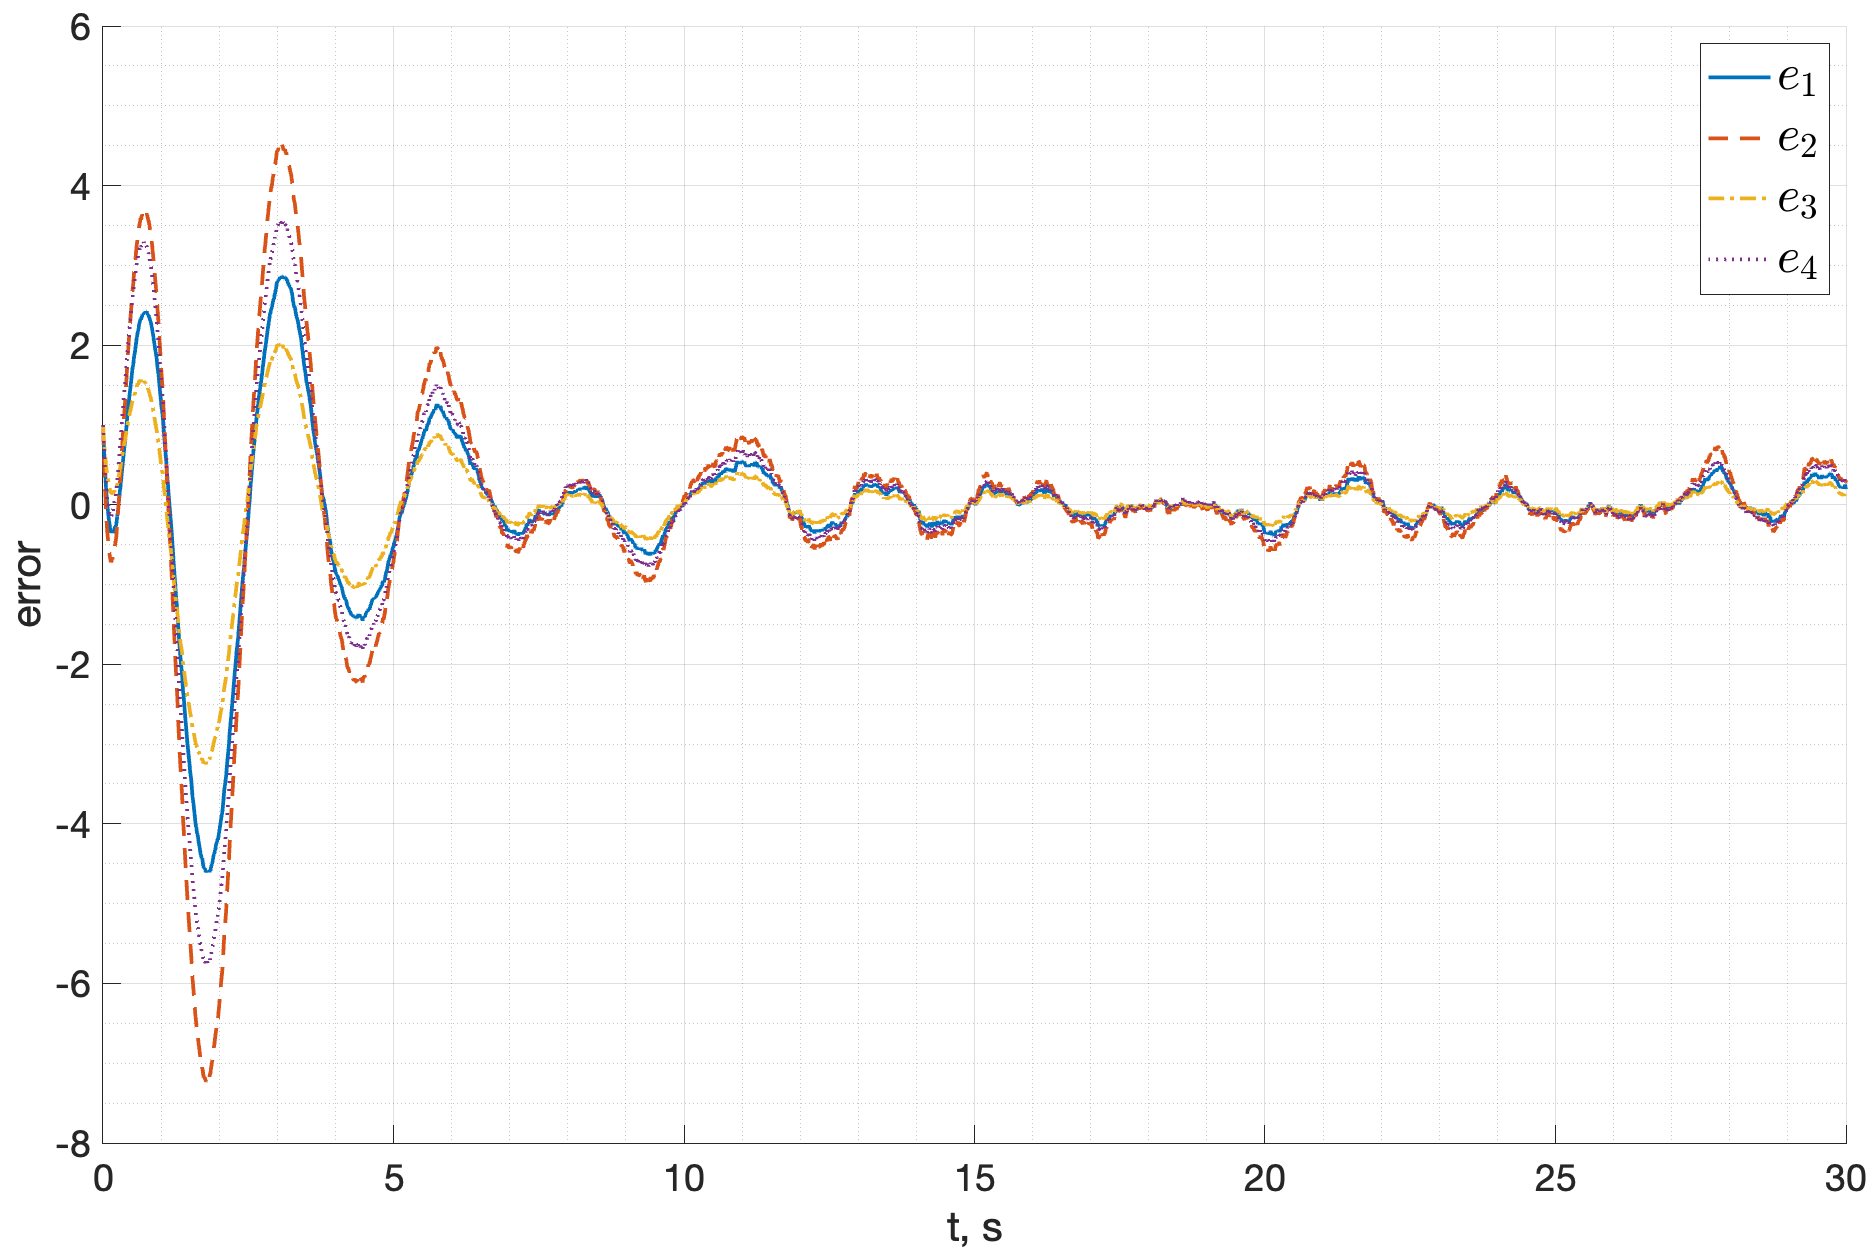
\includegraphics[width=\textwidth]{media/plots/kalman_task2/err_1.png}
    \caption{Ошибка оценки состояния фильтром Калмана $L_1$}
    \label{fig:kalman1_err}
\end{figure}
\begin{figure}[ht!]
    \centering
    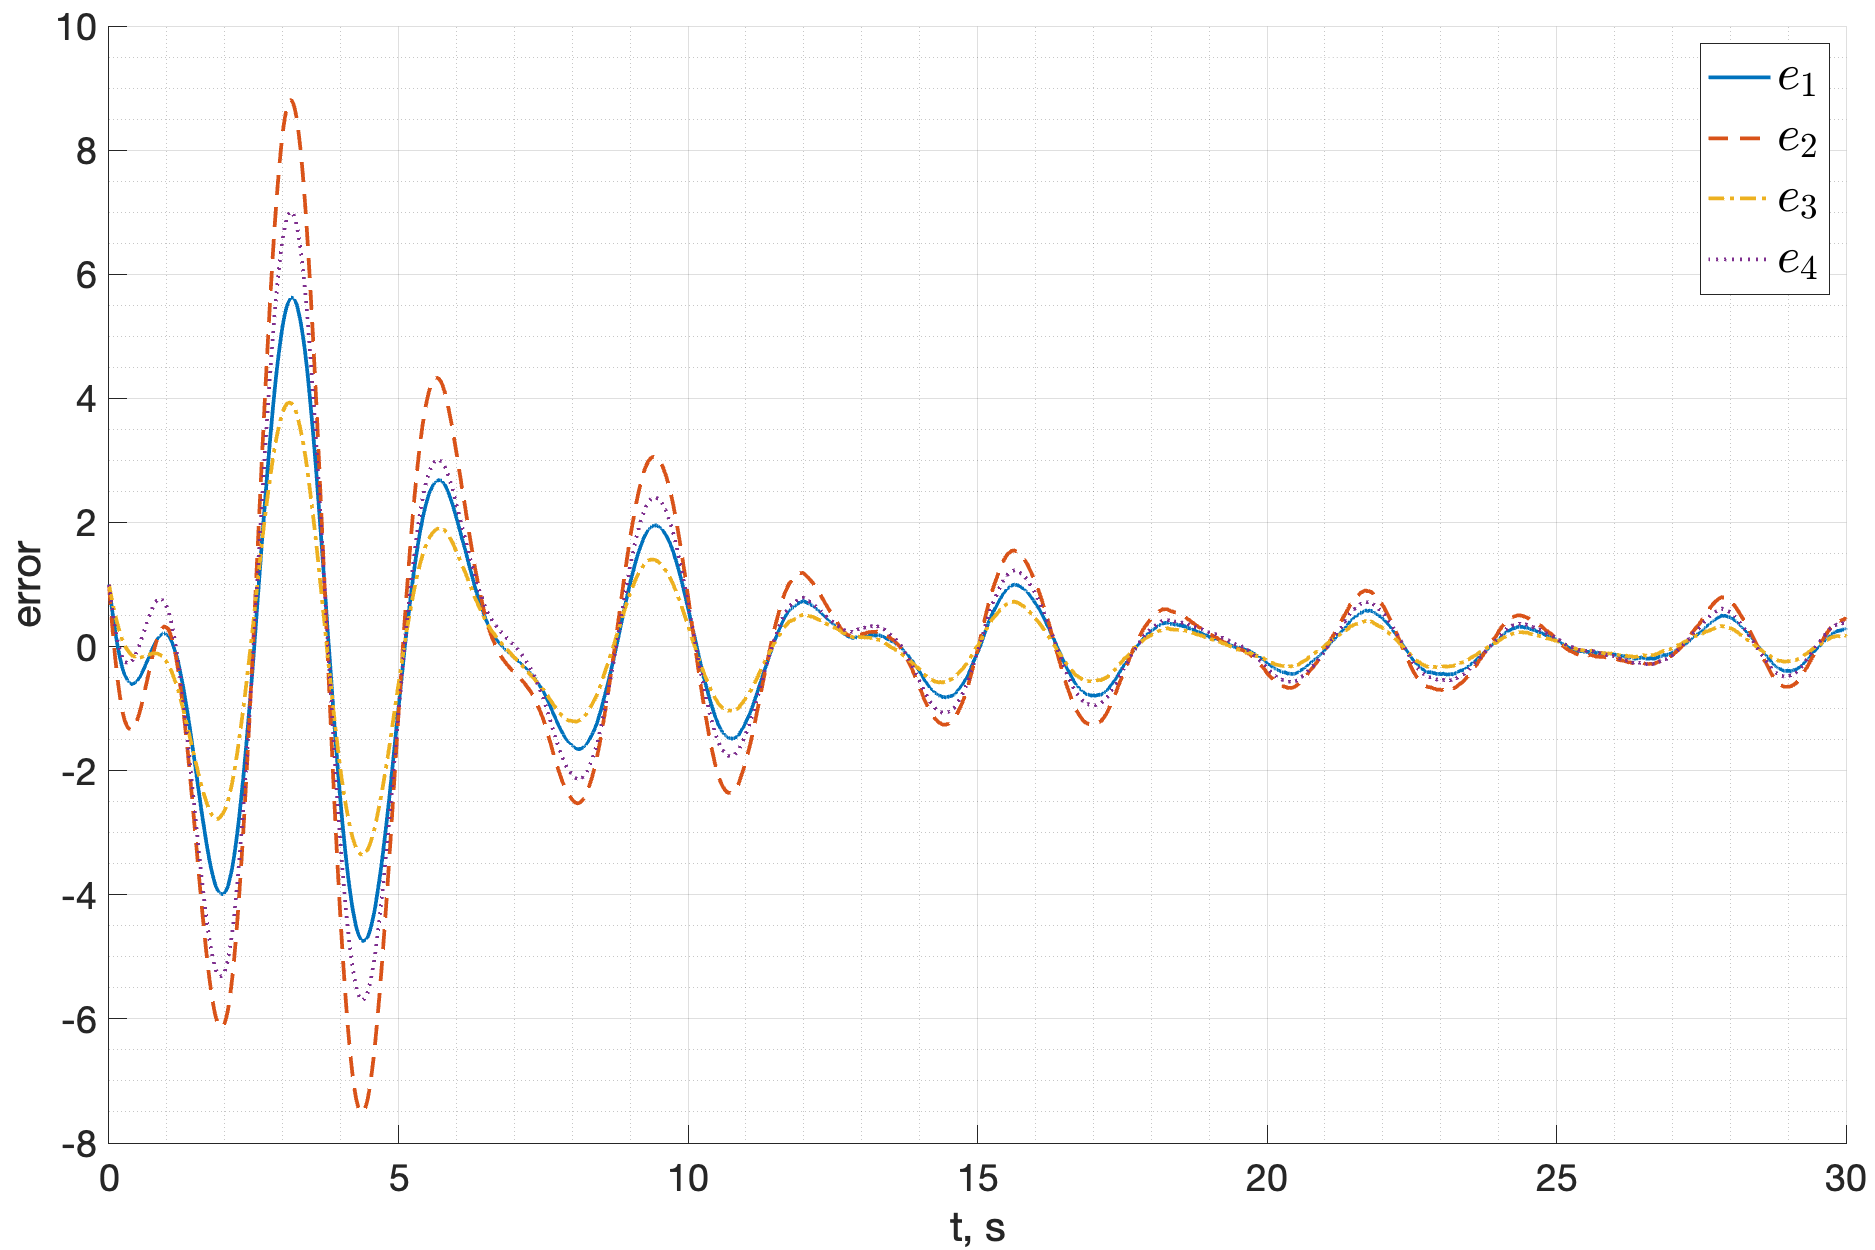
\includegraphics[width=\textwidth]{media/plots/kalman_task2/err_2.png}
    \caption{Ошибка оценки состояния фильтром Калмана $L_2$}
    \label{fig:kalman2_err}
\end{figure}
\begin{figure}[ht!]
    \centering
    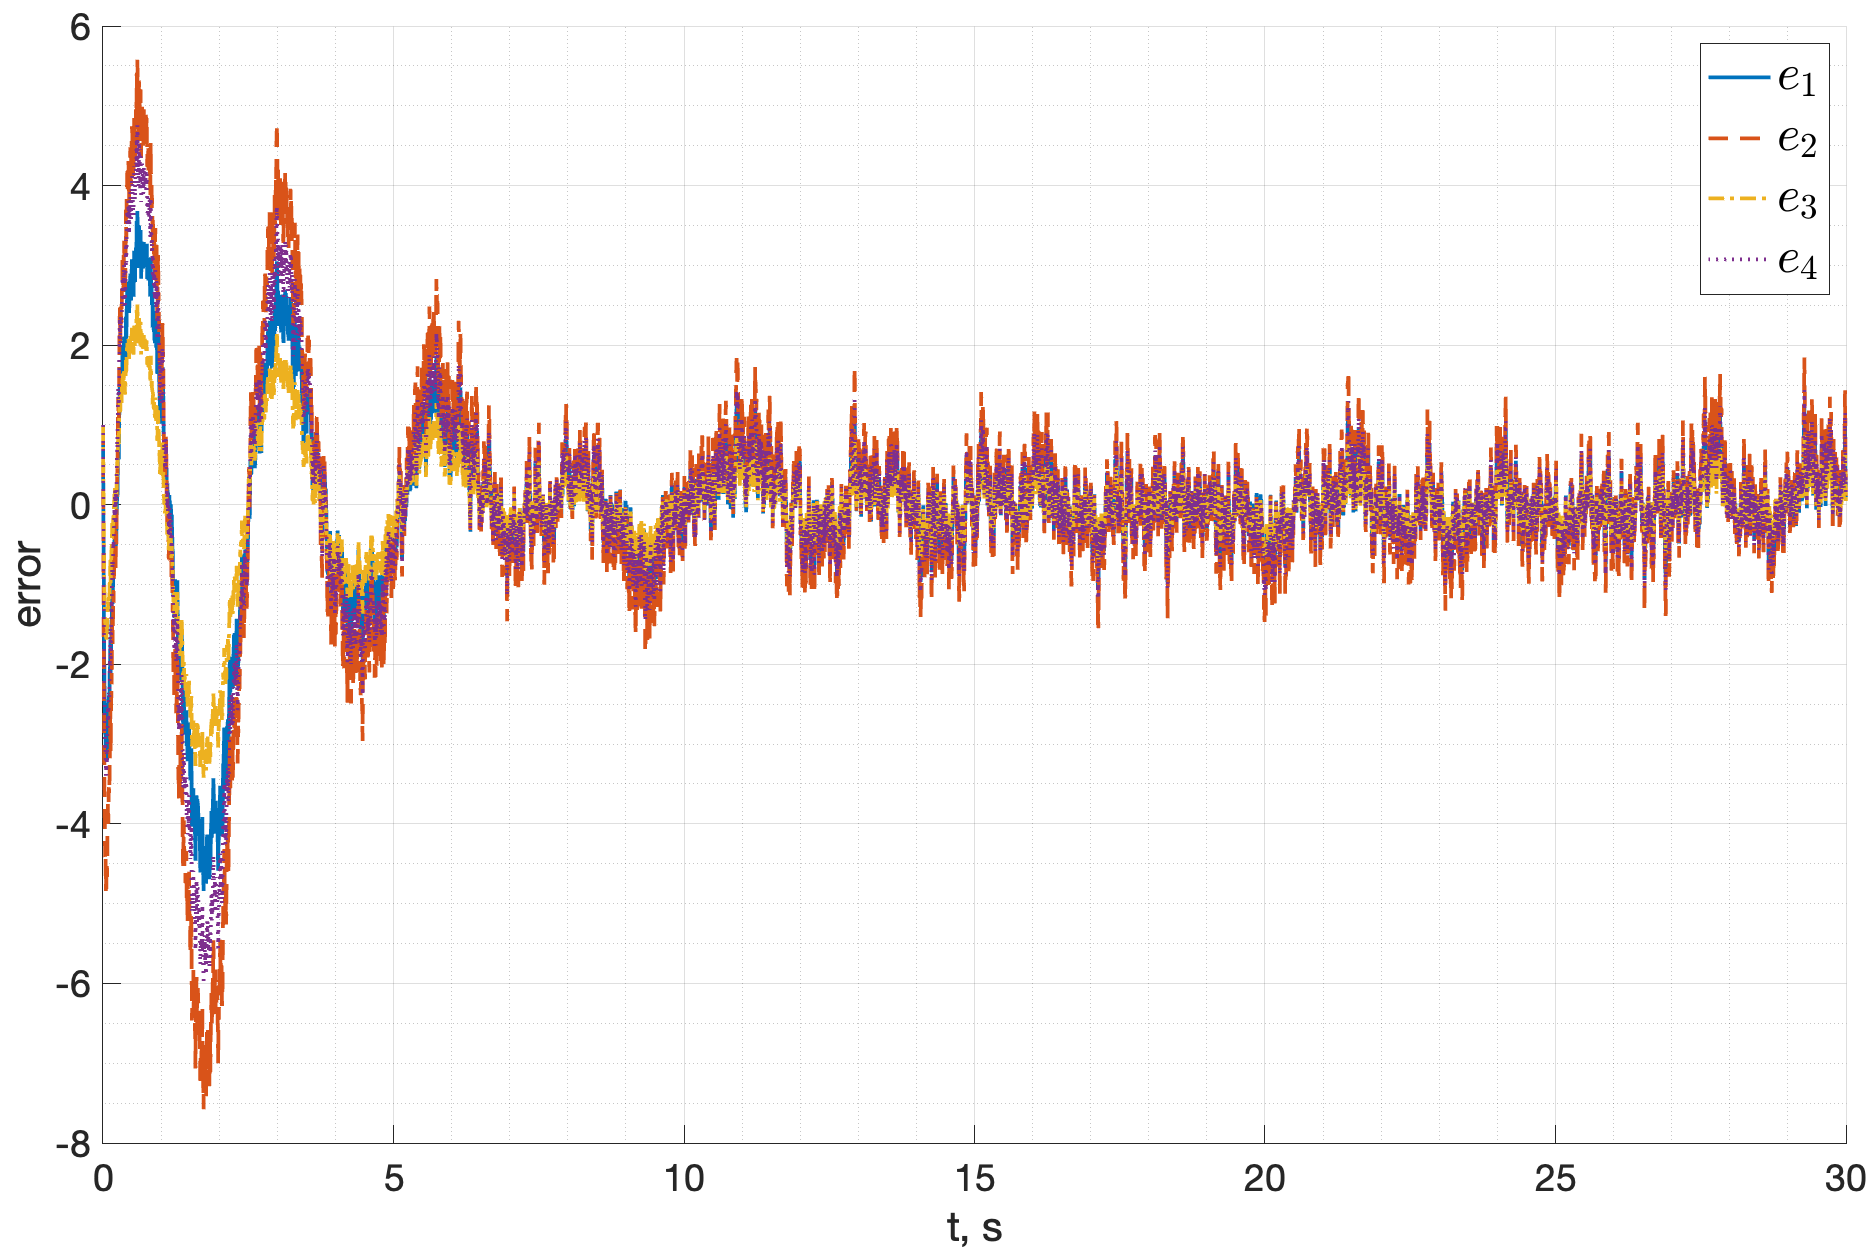
\includegraphics[width=\textwidth]{media/plots/kalman_task2/err_3.png}
    \caption{Ошибка оценки состояния фильтром Калмана $L_3$}
    \label{fig:kalman3_err} 
\end{figure}
\begin{figure}[ht!]
    \centering
    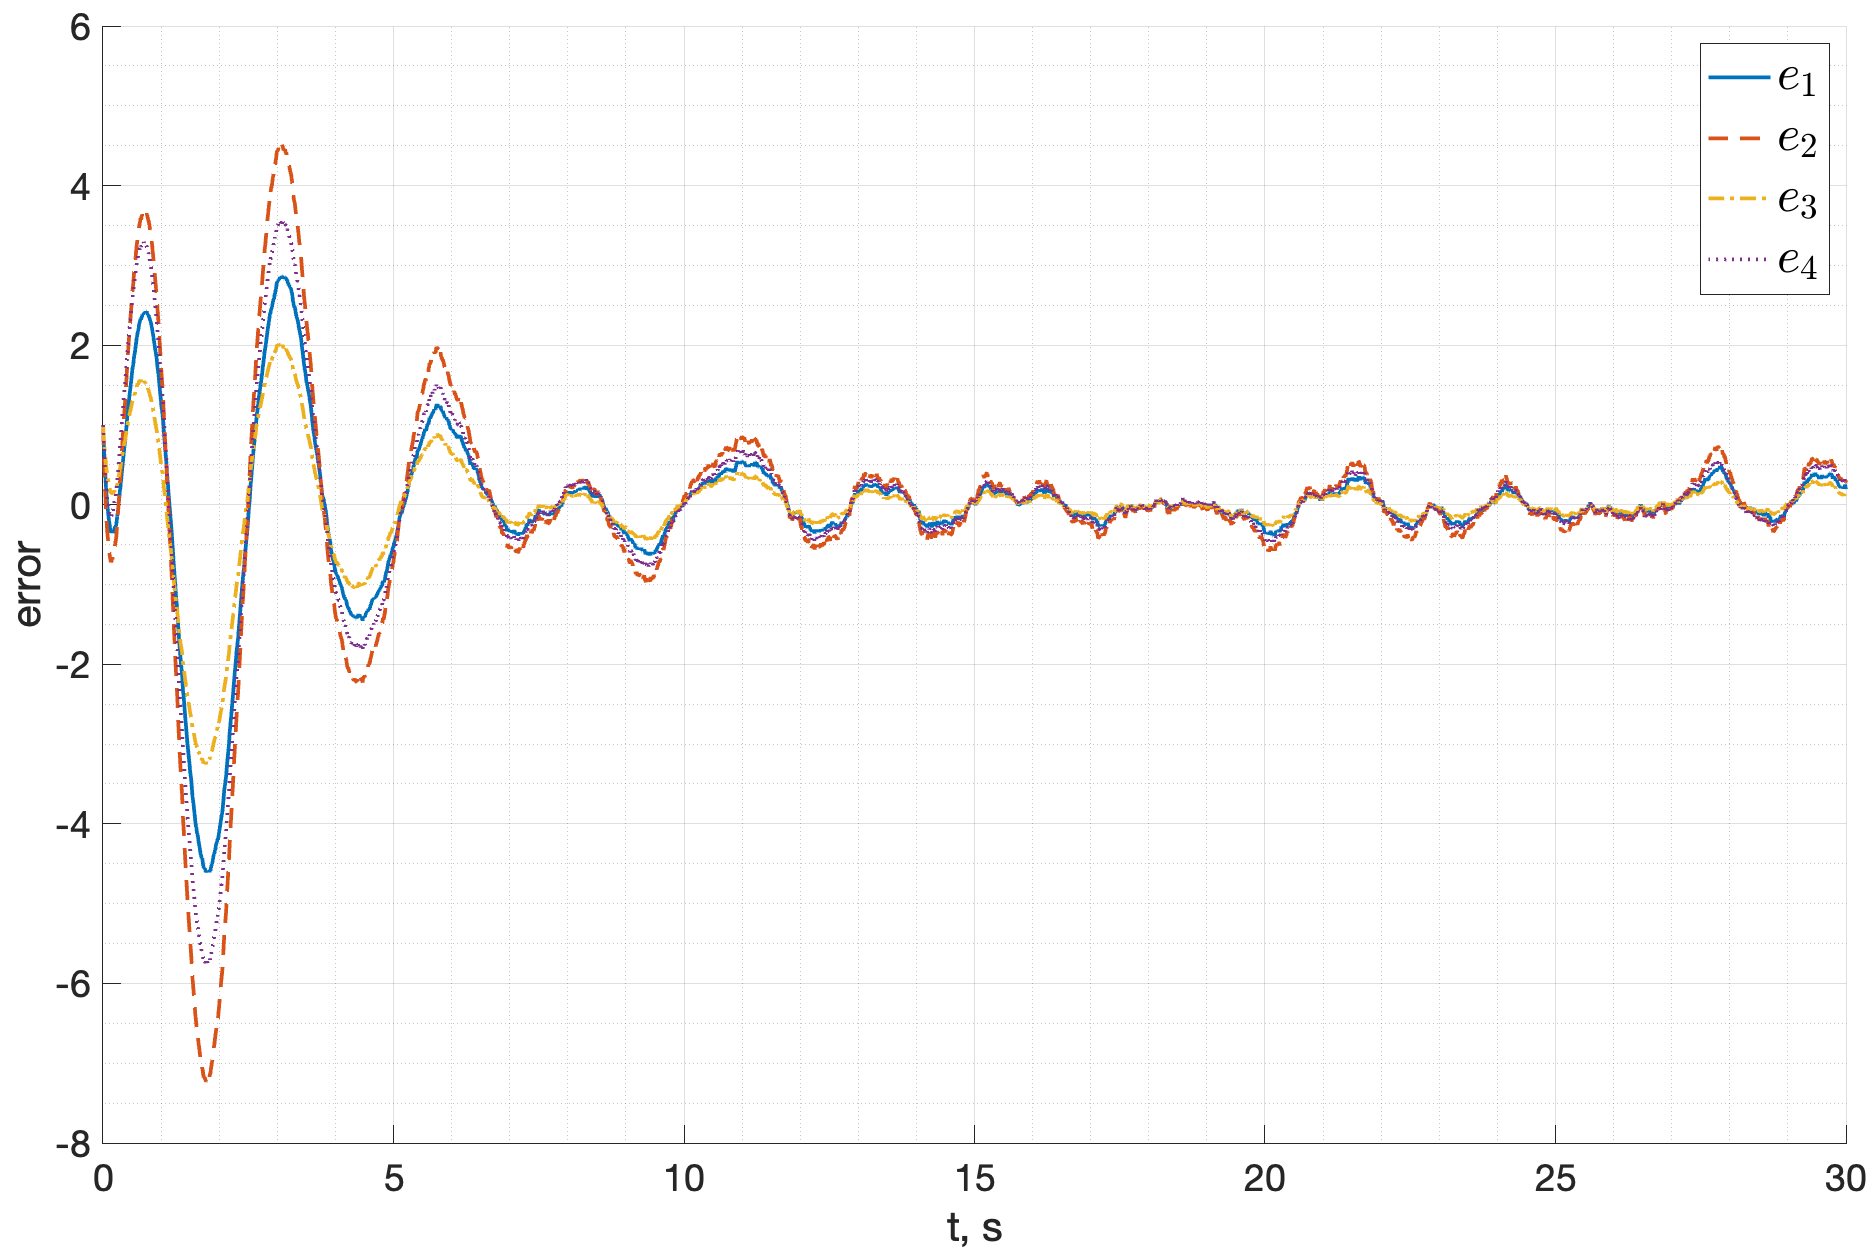
\includegraphics[width=\textwidth]{media/plots/kalman_task2/err_4.png}
    \caption{Ошибка оценки состояния фильтром Калмана $L_4$}
    \label{fig:kalman4_err}
\end{figure}
   

\FloatBarrier
\subsection{Выводы}
Как и с LQR можно сказать, что вклад вносит не каждая матрица весов по отдельности, а их сочетание.
Наиболее заметный шум в оценке системы получился при \textit{сильной} матрице веса $Q$ и
\textit{слабой} матрице веса $R$. При этом, ни в одном из случаев не удалось полностью 
избавиться от шума в оценке состояния системы. Это связано с тем, что наблюдатель 
не имеет сведений о шуме в системе, как это было в случае использования принципа внутренней 
модели в прошлых работах. Тем не менее, сравнивая величину шумов в выходе системы и в оценке состояния,
можно заметить, что фильтр Калмана позволяет существенно уменьшить внешние возмущения и помехи. 